\documentclass[aspectratio=169,11pt]{beamer}
% Shared preamble for the CogLean decks.
% Build the slides alone, or with speaker notes (see the Makefile):
%   pdflatex deck.tex                                   -> slides
%   pdflatex -jobname=deck-notes "\def\withnotes{}\input{deck.tex}"  -> slides + notes
\usetheme{default}
\usecolortheme{seahorse}
\setbeamertemplate{navigation symbols}{}
\setbeamertemplate{footline}[frame number]
\setbeamerfont{note page}{size=\small}
\ifdefined\withnotes
  \setbeameroption{show notes}
\fi
\usepackage[T1]{fontenc}
\usepackage{lmodern}
\usepackage{booktabs}
\usepackage{amsmath,amssymb}
\usepackage{tikz}
\usetikzlibrary{positioning,arrows.meta,shapes.misc}
\tikzset{
  box/.style={draw, rounded corners, align=center, minimum height=8mm, inner sep=4pt, fill=blue!6},
  arr/.style={-{Stealth[length=2mm]}, thick}
}
\newcommand{\code}[1]{\texttt{#1}}
\newcommand{\has}{\textbf{has}}
\newcommand{\lacks}{\textcolor{red!70!black}{lacks}}
\newcommand{\never}{\textcolor{red!70!black}{\textbf{never}}}
\newcommand{\canhold}{can hold}


\title{Knowledge, concepts, and views}
\subtitle{One knowledge model; rival theories of semantic memory and concepts, compared by proof}
\author{Jeff Shrager}
\date{October 2026}

\begin{document}

\begin{frame}
  \titlepage
\end{frame}
\note{
This talk is about knowledge in CogLean. Until now the library has been about memory and retrieval. Here I'll describe one knowledge model, semantic nets whose nodes are terms, and show three theories built on it: two rival theories of semantic memory, a theory of conceptual combination, and my own 1987 theory of view application. They're compared the same way the memory families are: phenomena stated as laws, and a matrix of which theory has which. The payoff is a result none of them gives alone: a view that turns graded, over-extended number concepts into exact ones, while leaving typicality untouched.
}

\begin{frame}{One knowledge model}
  \begin{itemize}
    \item A \textbf{knowledge net}: labelled links between nodes; one label is the hierarchy (\emph{isa}).
    \item Nodes are \textbf{terms}: atoms (\emph{canary}), structured values (\emph{set the program-plan to MOVE FORWARD 9}), and typed \emph{holes} (\emph{a Real-World-Action}).
    \item \textbf{Everything is links}: frames and slots, patterns, a concept's prototype (its votes), and even \emph{how} a concept decides membership.
    \item \textbf{Processes are generic}: inheritance, verification, prototype similarity, categorization, view application. A theory supplies data and choices, not a new representation.
  \end{itemize}
\end{frame}
\note{
First, the representation. A knowledge net is a set of labelled links between nodes, with one label for the hierarchy. The nodes are terms: atoms like canary, structured values like "set the program-plan to move forward nine", and typed holes, unfilled places like "a real-world action". Everything a theory knows is links: frames and their slots, patterns, a concept's prototype with its votes, and even the method a concept uses to decide membership. The processes that run on it are generic and proved once in the library. A theory supplies data and a few choices, not a new representation. That's what makes it a foundation rather than a set of separate models.
}

\begin{frame}{Semantic nets: what is proved for every net}
  \begin{columns}
    \column{0.42\linewidth}
    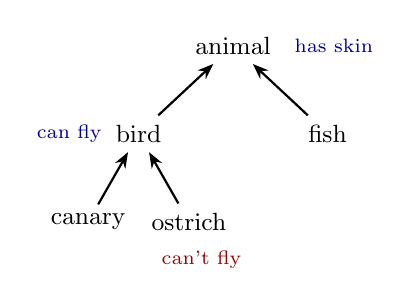
\begin{tikzpicture}[scale=0.8, every node/.style={font=\small}]
      \node (an) at (1.5,3) {animal};
      \node (bi) at (0,1.6) {bird};
      \node (fi) at (3,1.6) {fish};
      \node (ca) at (-0.8,0.2) {canary};
      \node (os) at (0.8,0.2) {ostrich};
      \draw[arr] (bi) -- (an); \draw[arr] (fi) -- (an);
      \draw[arr] (ca) -- (bi); \draw[arr] (os) -- (bi);
      \node[font=\scriptsize, text=blue!60!black] at (3.1,3.0) {has skin};
      \node[font=\scriptsize, text=blue!60!black] at (-1.1,1.6) {can fly};
      \node[font=\scriptsize, text=red!60!black] at (1.0,-0.4) {can't fly};
    \end{tikzpicture}
    \column{0.55\linewidth}
    \begin{itemize}
      \item \textbf{Inheritance}: a property stored once at a superordinate is found by every subordinate (cognitive economy).
      \item \textbf{Override}: a single-valued property stored nearer wins (an ostrich can't fly).
      \item \textbf{Accumulation}: many-valued properties collect up the hierarchy (a canary has wings \emph{and} skin).
      \item \textbf{Distance}: the least number of \emph{isa} links.
    \end{itemize}
  \end{columns}
\end{frame}
\note{
The base layer is the semantic net, and its theorems hold for every net. A property stored once at a superordinate is found by every subordinate: that's cognitive economy. A single-valued property stored nearer overrides one higher up, so the ostrich can't fly though birds can. Many-valued properties accumulate: a canary has wings from bird and skin from animal. My first version got this wrong, stopping at the first level that stored any "has" property, so a canary had no skin. The canary test caught it, which is what the worked examples are for. And the distance between two concepts is the least number of isa links between them.
}

\begin{frame}{Two theories of semantic verification}
  \small
  \begin{columns}[T]
    \column{0.48\linewidth}
    \textbf{Hierarchical network}\\(Collins \& Quillian 1969)
    \begin{itemize}
      \item Move up from the subject, searching properties at each node.
      \item Each move and each retrieval costs; costs add.
      \item Cost depends only on \emph{where} things are stored.
    \end{itemize}
    \column{0.48\linewidth}
    \textbf{Feature comparison}\\(Smith, Shoben \& Rips 1974)
    \begin{itemize}
      \item Stage 1: overall similarity of feature lists; very high, \emph{true}; very low, \emph{false}.
      \item Otherwise stage 2: compare defining features only.
      \item Cost depends on \emph{similarity}.
    \end{itemize}
  \end{columns}
  \bigskip
  Costs are \textbf{ordinal}, steps or stages: the theories disagree about the \emph{order} of verification times, and that is what is proved.
\end{frame}
\note{
On these nets, two classic rival theories of how people verify "a canary is a bird". Collins and Quillian's hierarchical network moves up from the subject, searching properties at each node, and every move and retrieval costs time, additively. So cost depends only on where things are stored. Smith, Shoben and Rips's feature comparison model compares feature lists: very high overall similarity says true at once, very low says false, and otherwise a second stage checks only the defining features. So cost depends on similarity. I count costs in steps or stages, not milliseconds: the theories disagree about the order of times, and that's what gets proved.
}

\begin{frame}{Laws of verification}
  Stated for \emph{any} verifier, against a hierarchy that says what is true:
  \begin{itemize}
    \item \textbf{Distance effect}: the farther category costs more (\emph{a canary is an animal} after \emph{a canary is a bird}).
    \item \textbf{Typicality effect}: two instances equally far below a category, verified at different costs (\emph{robin} faster than \emph{chicken}).
    \item \textbf{Reversal}: an instance verified faster as a member of the farther category (\emph{a chicken is an animal} faster than \emph{a chicken is a bird}).
  \end{itemize}
  \bigskip
  Proved once: a reversal contradicts the distance effect.
\end{frame}
\note{
As with memory, the phenomena are laws, stated for any verifier. The distance effect: a farther category costs more. The typicality effect: two instances equally far below a category, like robin and chicken under bird, verified at different costs. And a reversal: an instance verified faster as a member of the farther category, as when a chicken is an animal is faster than a chicken is a bird. One theorem relates them: a reversal contradicts the distance effect.
}

\begin{frame}{The semantic-memory matrix}
  \begin{center}
  \begin{tabular}{lccc}
    \toprule
    & Distance & Typicality & Reversal\\
    \midrule
    Hierarchical (C\&Q) & \has & \never & \never\\
    Feature comparison (SSR) & \lacks & \canhold & \canhold\\
    \midrule
    People (RSS 1973; SSR 1974) & mostly & yes & yes\\
    \bottomrule
  \end{tabular}
  \end{center}
  \begin{itemize}
    \item C\&Q's cells hold for \emph{every} net: cost is distance, so equally distant instances always cost the same.
    \item The feature model shows both effects with bird features; for every setting, a more similar instance is never slower.
    \item C\&Q's Figure~1 gives the six sentence types of Fig.~2 in the paper's order.
  \end{itemize}
\end{frame}
\note{
Here's the matrix. The hierarchical model has the distance effect for every net, and can never produce a typicality effect or a reversal, at any setting, because its cost is exactly the distance. The feature model shows both effects with a set of bird features, and so lacks the distance effect; and for every setting, a more similar instance is never slower. The evidence, typicality effects and reversals, refutes the hierarchical model's never cells, which is the history of the field written as theorems. As a faithfulness check, Collins and Quillian's own Figure 1 gives their six sentence types in the order of their Figure 2.
}

\begin{frame}{Concepts: combination and over-extension}
  \begin{itemize}
    \item \textbf{Selective modification} (Smith, Osherson, Rips \& Keane 1988): \emph{red} shifts the color votes of \emph{apple} to red and boosts color's diagnosticity.
    \item \textbf{Threshold membership} (Hampton 2007): membership is a nondecreasing function of the same similarity.
    \item Proved for every setting: the \textbf{conjunction effect}, hence \textbf{over-extension} (more a member of \emph{red apple} than of \emph{apple}).
    \item The paper's figures reproduced exactly.
  \end{itemize}
  \bigskip
  Prototypes are links in the knowledge net, so these theorems apply to any concept held there.
\end{frame}
\note{
Concepts. The selective modification model combines an adjective with a noun by modifying the noun's prototype: red moves apple's color votes onto red and makes color more diagnostic. With Hampton's threshold model, membership is a nondecreasing function of the same similarity. Proved for every setting: the conjunction effect, and from it over-extension, being more a member of red apple than of apple, which fuzzy logic forbids. The paper's figures come out exactly. And because prototypes are just links in the knowledge net, these theorems apply to any concept held there.
}

\begin{frame}{The trouble with numbers}
  \begin{itemize}
    \item \emph{multiple of 3}, learned from 3, 6, \dots, 30; \emph{even multiple of 3} by modification.
    \item 14 is an \emph{even multiple of 3} to degree $.80$, a \emph{multiple of 3} to $.06$.
    \item \textbf{Incoherent}: more a member of the combination than of its head.
    \item \textbf{False}: Lean proves 14 is not a multiple of 3.
  \end{itemize}
  \bigskip
  People know better. So for numbers, something replaces similarity as the arbiter of membership, without removing the prototype.
\end{frame}
\note{
Now the problem. Learn multiple of three from the exemplars three through thirty, and form even multiple of three by modification. Then fourteen is an even multiple of three to degree point eight and a multiple of three to degree point oh six. That's incoherent, and Lean proves it false. People know better: for numbers, something other than similarity decides membership. But it can't simply delete the prototype, because people still find some even numbers more typical than others. My 1987 theory of view application offers a mechanism.
}

\begin{frame}{View application (Shrager 1987)}
  A \emph{view} is an abstract schema from outside the domain. Applying it to a theory:
  \begin{enumerate}
    \item \textbf{copy} the view;
    \item \textbf{merge} the theory: match type frames by abstract type, or at random within a kind; the view wins on matched slots;
    \item \textbf{coerce} re-parented instances through their old and new parents' patterns;
    \item \textbf{bind} the view's holes from the theory;
    \item \textbf{single function}: an object bound to one operation leaves the others.
  \end{enumerate}
  \medskip
  Random ties, never revisited: application gives a \emph{distribution} over theories. Proved for every view and theory: the view is kept, the view wins on matched frames, unmatched frames survive, instances are re-parented.
\end{frame}
\note{
View application is the mechanism from my 1987 Machine Learning paper. A view is an abstract schema from outside the domain, such as programmable device or clock time. Applying it copies the view, merges the theory in, matching frames by type, and on a match the view wins, which makes the change non-monotonic. Re-parented instances are coerced through their old and new parents' patterns, the view's holes are bound from the theory, and an object bound to one operation leaves the others. The paper resolves ambiguity at random and never revisits it, so here application gives a distribution over theories. The general properties are proved for every view and theory.
}

\begin{frame}{Faithfulness: the paper's Table 4}
  \begin{itemize}
    \item Tables 1 and 2 of the paper as data: a BigTrak theory and the CODE.AND.STARTUP view.
    \item Applying the view gives \textbf{Table 4 exactly}, with probability $1/2$.
    \item The other half: \emph{Action-operation} matched to \emph{Immediate-operation} instead of \emph{Memory-operation}, the random choice the paper describes.
    \item \emph{Do (MOVE FORWARD 9)} becomes \emph{Set the program-plan to (MOVE FORWARD 9)} by coercion; GO leaves Sequence-1; the script runs the memory operation, then the immediate one.
  \end{itemize}
  \bigskip
  All five steps are the library's; BigTrak is only data.
\end{frame}
\note{
Is the formalization faithful? The paper works one example: Tables 1 and 2 are a theory of the BigTrak toy and the code-and-startup view, and Table 4 is the result. Given the two tables as data, the generic process gives Table 4 exactly, half the time. The other half, action-operation is matched to immediate-operation instead, which is exactly the random choice the paper says it makes. You can see each step at work: coercion turns "do move forward nine" into "set the program-plan to move forward nine", GO leaves the sequence, and the script now runs the memory operation and then the immediate one.
}

\begin{frame}{An ARITHMETIC view for number concepts}
  \begin{columns}[T]
    \column{0.48\linewidth}
    \textbf{The learner's theory}
    \begin{itemize}
      \item \emph{category}: membership by similarity (threshold); combination by modification.
      \item \emph{multiple of 3}, \emph{even}: prototypes learned from exemplars.
    \end{itemize}
    \column{0.48\linewidth}
    \textbf{The ARITHMETIC view}
    \begin{itemize}
      \item \emph{category}: membership by divisibility (divisor from the concept's name); combination by conjunction.
    \end{itemize}
  \end{columns}
  \bigskip
  Applying it: \emph{category} matches \emph{category}, so the view's test and combination win. The concepts' prototypes are not matched, so they are \textbf{kept}.
\end{frame}
\note{
Now apply a view to number concepts. In the learner's theory, the category type frame decides membership by similarity with a threshold, and combines by modification; multiple of three and even have prototypes learned from exemplars. The arithmetic view has its own category frame: membership by divisibility, with the divisor read from the concept's name, and combination by conjunction. Applying it with exactly the same process as the BigTrak: category matches category, so the view's test and combination win. The concepts' own frames, with their prototypes, aren't matched, so they're kept.
}

\begin{frame}{Before and after the view}
  \small
  \begin{center}
  \begin{tabular}{lll}
    \toprule
    & Before & After\\
    \midrule
    14 in \emph{multiple of 3} & $.06$ & $0$\\
    14 in \emph{even multiple of 3} & $.80$ (over-extension) & $0$\\
    \emph{even multiple of 3} & similarity, modified prototype & \textbf{exactly} $6 \mid n$, every $n$\\
    Over-extension & at 14 & \textbf{never}, at any $n$\\
    Typicality & & \textbf{unchanged}, every $n$\\
    \bottomrule
  \end{tabular}
  \end{center}
  \begin{itemize}
    \item \textbf{Dissociation}: 14 as an \emph{even multiple of 3} is more typical ($-16$) than 9 as a \emph{multiple of 3} ($-23$), yet only 9 is a member. Before the view, impossible: membership is a nondecreasing function of typicality.
    \item Graded typicality for an all-or-none concept: Armstrong, Gleitman \& Gleitman (1983), \emph{odd number}.
  \end{itemize}
\end{frame}
\note{
Here's the result. Before the view, fourteen is over-extended. After it, membership in even multiple of three is exactly divisibility by six, proved for every number, so there's no over-extension anywhere. And typicality is unchanged for every number, because the view never touched the prototypes. So typicality and membership come apart: fourteen as an even multiple of three is more typical than nine as a multiple of three, yet only nine is a member. Before the view that's impossible, and it's a theorem: when membership is a nondecreasing function of typicality, a more typical judgment is never less a member. That's what Armstrong, Gleitman and Gleitman found for odd number: people rate some odd numbers as better examples, while insisting membership is all or none. Here it's a derived result.
}

\begin{frame}{Choosing the view: spreading activation}
  The 1987 paper had no principled account of \emph{which} view to apply. Collins \& Loftus (1975) supply one:
  \begin{itemize}
    \item Activation starts at the \textbf{cue} (a key's label) and at the \textbf{concepts the current theory uses}.
    \item It spreads along links, each passing on a fraction set by its strength; activation from different sources \textbf{sums}.
    \item A view is chosen in proportion to its activation, then \textbf{applied}.
  \end{itemize}
  \medskip
  Proved for every net: activation sums over sources; it is never negative; priming never lowers it; priming a candidate never lowers its share.
  \medskip

  The composition is a mixture, chance of choosing a view times chance of each result: the shape of recognition-then-retrieval in the multi-digit model.
\end{frame}
\note{
View application needs a view, and the 1987 paper had no principled account of how one is chosen: views were suggested by key labels, by the device's behavior, or by the current theory. Collins and Loftus's spreading activation supplies one, on the same net. Activation starts at the cue, say a key's label, and at the concepts the learner's theory already uses. It spreads along links, each passing on a fraction set by its strength, and activation from different sources adds up. A view is chosen in proportion to its activation and then applied. The general facts are proved for every net: activation sums, it's never negative, and priming never lowers it or a candidate's share. Put together, it's a mixture, like recognition followed by retrieval in the multi-digit model.
}

\begin{frame}{Same key, different knowledge}
  A hypothetical device with a key labelled ``+'':
  \begin{itemize}
    \item ``+'' suggests CALCULATING (``+'' adds to the display), and more weakly PROGRAMMING (``+'' appends a step).
    \item \emph{Memory} suggests PROGRAMMING.
  \end{itemize}
  \begin{center}
  \begin{tabular}{lcc}
    \toprule
    Learner's theory & ``+'' adds & ``+'' appends a step\\
    \midrule
    no memory & $2/3$ & $1/3$\\
    has a memory & $2/5$ & $3/5$\\
    \bottomrule
  \end{tabular}
  \end{center}
  The same cue brings in different knowledge, depending on what the learner already knows. Strengths are illustrative; the composition is general.
\end{frame}
\note{
Here's the example. A device has a key labelled plus. Plus suggests a calculating view, where it adds to the display, and more weakly a programming view, where it appends a step. And memory suggests programming. A learner whose theory has no memory reads plus as adding two thirds of the time. A learner who has already learned that the device has a memory, as after the code-and-startup view, reads it as appending a step three fifths of the time, because activation from memory adds to what the cue sends to programming. The same cue brings in different knowledge depending on what the learner already knows. The numbers are illustrative; the composition is general.
}

\begin{frame}{The concept matrix}
  \scriptsize
  \begin{center}
  \setlength{\tabcolsep}{4pt}
  \begin{tabular}{lcccccc}
    \toprule
    & Distance & Typicality & Reversal & Conj.\ effect & Over-ext. & Dissociation\\
    \midrule
    Hierarchical net & \has & \never & \never & -- & -- & --\\
    Feature comparison & \lacks & \canhold & \canhold & -- & -- & --\\
    Selective modification & -- & -- & -- & \has & \has & \never\\
    \quad + ARITHMETIC view & -- & -- & -- & \has & \never & \canhold\\
    \midrule
    People & mostly & yes & yes & yes & yes & yes\\
    \bottomrule
  \end{tabular}
  \end{center}
  \normalsize
  \begin{itemize}
    \item \has/\never: every setting (conditions stated). \lacks/\canhold: one setting. --: not stated for that theory.
    \item Without a view, membership never goes against typicality (any nondecreasing threshold); with it, over-extension never occurs for number concepts.
  \end{itemize}
\end{frame}
\note{
Putting it together, the concept matrix. The verification theories are rows on the left, the combination theories on the right. The hierarchical net has the distance effect and never the other two; feature comparison lacks it and can show both. Selective modification has the conjunction effect and over-extension at every setting, and because membership is a nondecreasing function of typicality, it can never dissociate them: that's a theorem too. Add the arithmetic view and over-extension never occurs for number concepts, while the conjunction effect in typicality survives, so the dissociation becomes possible. The dashes are honest: those phenomena aren't stated for those theories yet. The people row is a judgment of the evidence, kept apart from the theorems as in the memory matrix.
}

\begin{frame}{What this adds, and next}
  \begin{itemize}
    \item \textbf{One model, many theories}: semantic memory, concept combination and theory change share nets, terms and processes; each theory is data and choices.
    \item \textbf{A rival-theory matrix for knowledge}, as for memory.
    \item \textbf{View application, formalized}: the paper's example exactly, a new consequence for concepts, and view selection by spreading activation.
  \end{itemize}
  \medskip
  Next:
  \begin{itemize}
    \item View selection by EPAM recognition of cues, as a rival to spreading activation; garden paths and their repair.
    \item Collins \& Loftus's decision process, making spreading activation a third verification family; feature lists as net links.
    \item Learning views; a cognitive-skills package (problem solving).
  \end{itemize}
\end{frame}
\note{
So what does this add? One knowledge model carrying several theories: semantic memory, conceptual combination and theory change share the same nets, terms and processes, and each theory is data plus a few choices. A matrix of rival theories for knowledge, like the one for memory. And view application formalized for the first time: the paper's own example comes out exactly, and applied to concepts it yields a consequence the 1987 paper never considered. Next: view selection by EPAM recognition of cues, as a rival to spreading activation, and garden paths, where a primed but wrong view is chosen and later repaired by failed predictions; Collins and Loftus's decision process, which would make spreading activation a third family of semantic memory; learning the views themselves; and a cognitive-skills package for problem solving.
}

\end{document}
